\documentclass[../Bachelorarbeit.tex]{subfiles}

\begin{document}
\label{sec:EFT}

\begin{figure}[h]
    \centering
    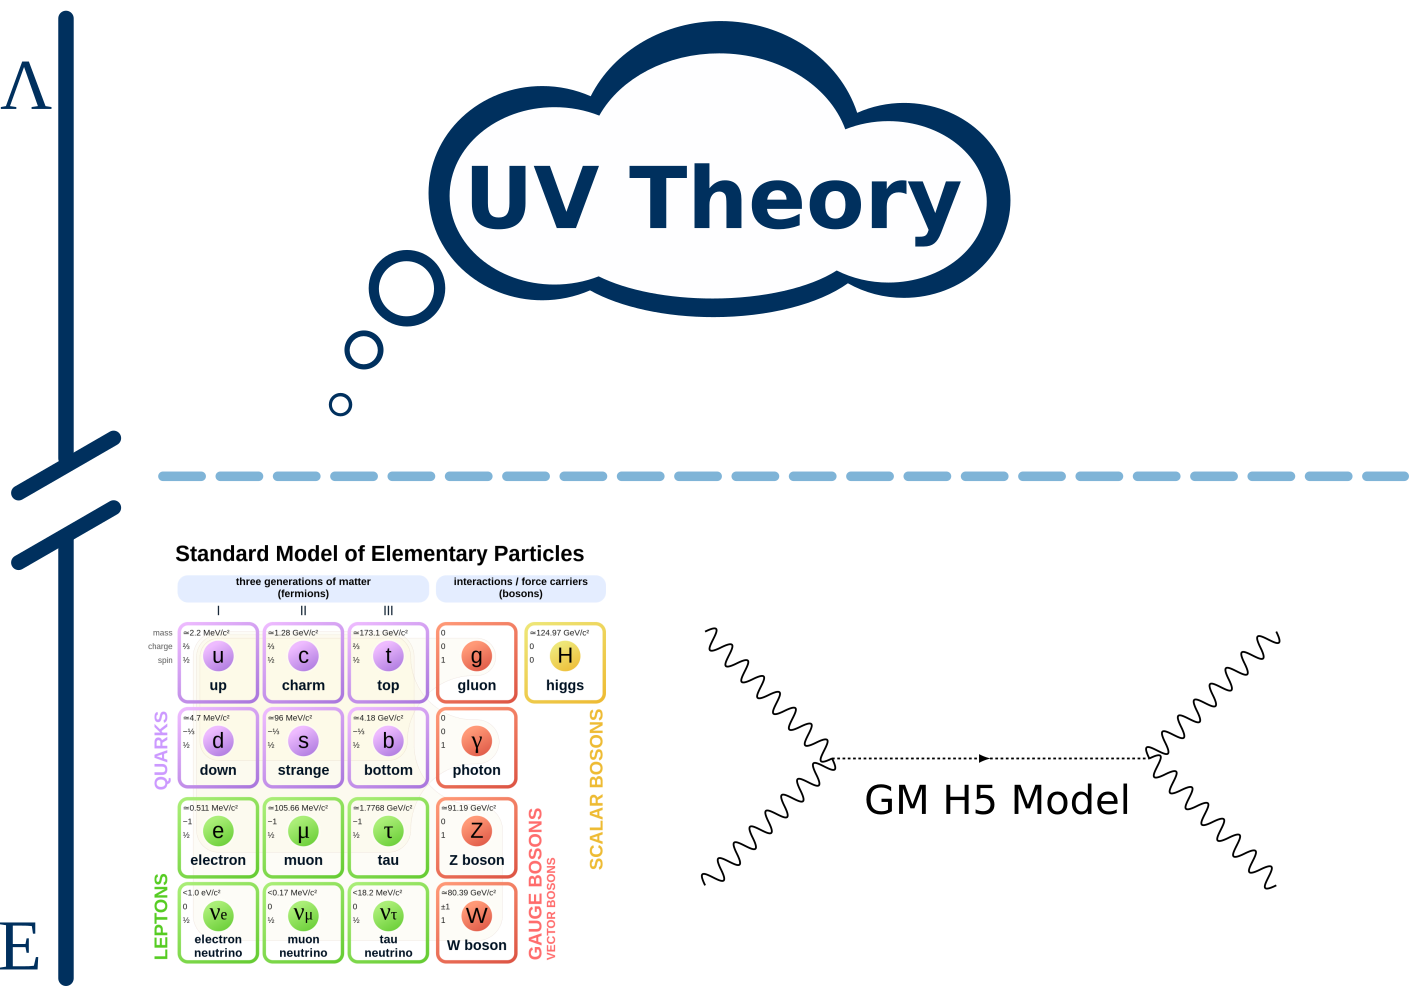
\includegraphics[width=0.5\textwidth]{images/EFT_Model.png}
    \caption{Sketch of the Basic EFT concept with the low energy observer having energy E and cutoff at $Lambda$. The SM and BSM theory(here GM H5 Model) are combined in the Effective Field Theory. \cite{Brivio.2017}}
    \label{fig:EFT_sketch}
\end{figure}

With the Standard Model Physicist try to describe the elementary Particles and interactions. It is successful in describing most processes in Biology, Chemistry, and Physics.
But the Standard Model is still incomplete. It can't describe Phenomenons like Gravity, Neutrino Masses, Matter-Antimatter asymmetry etc. This is where effective field theory comes in.
Here we look at the Standard Model as a low energy approximation of an underlying Ultraviolet Theory (figure~\ref{fig:EFT_sketch}).

%-------------------------------------------------------------------------------------Fermi Theory-------------------------------------------------------------------------------------------------------
\subsection{Fermi Theory on the example Tau Decay}
\label{sec:Fermi}
Enrico Fermi proposed 1933 the Fermi Theory in order to describe the $\beta$-decay. His theory was able to describe the
weak coupling quite well without the former knowledge about the $W^{\pm}$-Boson which was only later theorized in 1968 by Steven Weinberg, Sheldon Glashow and Abdus Salam.
The $W^{\pm}$-Boson was finally discovered in 1983. 50 years after Fermi's first successful description of an Interaction involving the $W^{\pm}$-Boson.
Today we would call the Fermi theory the low-energy effective field theory of $W^{\pm}$-Boson.
Let us now try to create our own Fermi Theory but instead of describing the $\beta$ decay we will look at the $\tau$-decay specifically the decay mode $\tau \rightarrow \nu_{\tau}e^{-}\nu_{e}$.
Even though we are technically cheating since Fermi didn't have our knowledge about the tensor structure of the Weak interaction in Quantum Field Theory or our knowledge about Feynman diagrams.
We will start by drawing the Feynamn Diagramm and writing down the Matrix element.
\begin{figure}[h]
    \centering
    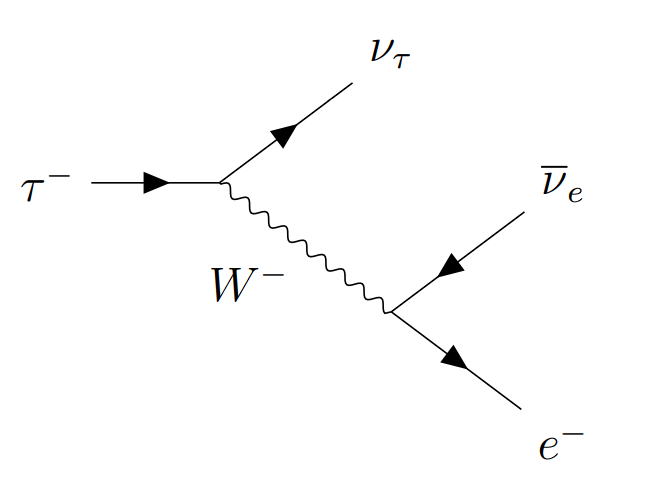
\includegraphics[width=0.5\textwidth]{images/Feynamn_tau_decay.PNG}
\end{figure}

\begin{equation}
    -i\mathcal{M}_{fi}= \left[ \frac{g_{W}}{\sqrt{2}} \overline{u}(k_{\nu_{\tau}})\frac{1}{2}\gamma^{\mu}(1-\gamma^{5})u(k_{\tau}) \right] \frac{g_{\mu\sigma}-\frac{k_{\nu}k_{\sigma}}{m_{W}^{2}}}{k^{2}-m_{W}^{2}} \left[ \frac{g_{W}}{\sqrt{2}} \overline{u}(k_{e})\frac{1}{2}\gamma^{\sigma}(1-\gamma^{5})v(k_{\overline{\nu_{e}}}) \right]
\end{equation}

In most low ernergy decay processes the momentum of the intermediate $W^{-}$-Boson is small compared to its mass. Therefore, we can approximate the
propagator(\ref{eq:Fermi_propergator}) in Orders of the momentum $k$ but we will be writing it in the Matrixelement in Orders
of mass since these are more interesting to us. In the Feynman Diagramm this can be expressed by collapsing the properagtor into a single Vertex.

\begin{figure}[h]
    \centering
    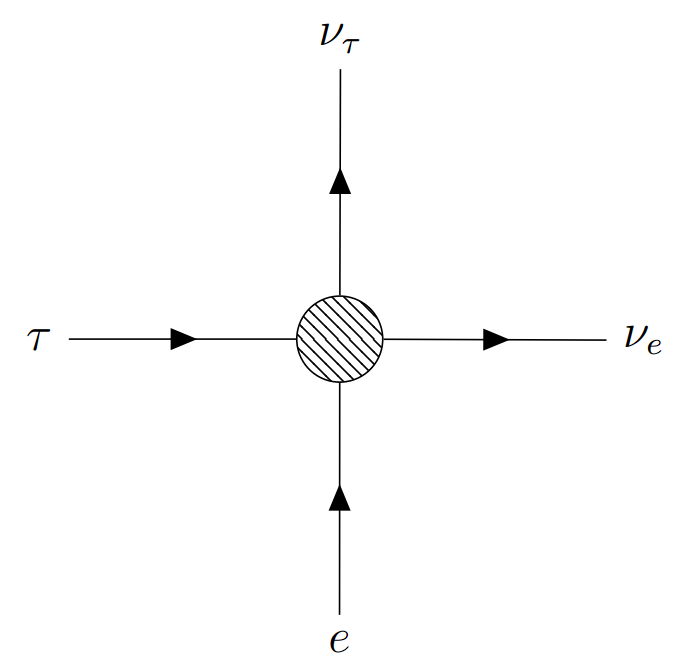
\includegraphics[width=0.5\textwidth]{images/propagator_collaps.PNG}
\end{figure}
\begin{equation}
    \frac{-ig_{\mu\sigma}-\frac{k_{\nu}k_{\sigma}}{m_{W}^{2}}}{k^{2}-m_{W}^{2}} \xrightarrow{\abs{q}^{2} \ll m_{W}^{2}} \frac{ig_{\mu\sigma}}{m_{W}^{2}} \left( 1 + \frac{k^{2}}{m_{w}^{2}}+\frac{k^{4}}{m_{W}^{6}}+\mathcal{O}(k^6) \right)
    \label{eq:Fermi_propergator}
\end{equation}

\begin{equation}
    \Rightarrow i\mathcal{M}_{fi}=\frac{g_{W}^{2}}{8 m_{W}^{2}} \left[ \overline{u}(k_{\nu_{\tau}})\gamma^{\mu}(1-\gamma^{5})u(k_{\tau}) \right] g_{\mu\sigma} \left[ \overline{u}(k_{e})\gamma^{\sigma}(1-\gamma^{5})v(k_{\overline{\nu_{e}}}) \right] + \mathcal{O}(m_{W}^{4})
    \label{eq:Fermi_colapse}
\end{equation}

Let us now compare our result with the result Fermi would have gotten if he knew about the parity violation discovered by Wu in 1957.

\begin{equation}
    i\mathcal{M}_{fi} = \frac{G_{F}}{\sqrt{2}} \left[ \overline{u}(k_{\nu_{\tau}})\gamma^{\mu}(1-\gamma^{5})u(k_{\tau}) \right] g_{\mu\sigma} \left[ \overline{u}(k_{e})\gamma^{\sigma}(1-\gamma^{5})v(k_{\overline{\nu_{e}}}) \right]
    \label{eq:Fermi_the_slim_Fermi}
\end{equation}
With $G_{F} \approx 4.5437957\times 10^{14} J^{-2}$ being the Fermi constant which is typically measured in the muon decay. The $1/\sqrt{2}$ is added in order to not change the numerical value of $G_{F}$ while considering the parity violation.
From equation \ref{eq:Fermi_colapse} and \ref{eq:Fermi_the_slim_Fermi} we get the following result.
\begin{equation}
    \frac{G_{F}}{\sqrt{2}} = \frac{g_{W}^{2}}{8 m_{W}^{2}}
\end{equation}
Defining the expansion scale $\Lambda=m_{W}$ and the Wilson coefficient $c= \frac{g_{W}^{2}}{8}$ we can see that the Matrix element has dimension 2.
With this we can also write down a new effective Lagrangian without the $W^{\pm }$-Boson but. The EFT described has to contain the tau, electron, their respective neutrienofields
as well as the Interaction Lagrangian.
\begin{equation}
    \mathcal{L}_{EFT} = \frac{c}{\Lambda^{2}} \left( \overline{\nu}_{\tau} \overline{\gamma}_{\rho} \tau \right) \left(\bar{e} \overline{\gamma}_{\rho} \nu_{e} \right) + \mathcal{O}(\frac{1}{\Lambda^{4}})
\end{equation}
Our Fermi Theory is only valid for low energies since Scattering Amplitude from the Standard Model and the EFT would
start to diverge once the Energy gets close to the mass of the $W^{\pm}$-Boson.
The $m_{W}$ defines the validity scale of the EFT in this case the Fermi Theory. For Energies higher than $m_{W}$the
Fermi Theory is no longer valid. We can increase the validity scale by including therms of higher dimension in $\Lambda$.
In this example we derived the Matrix element from the SM and then compared the result with the result from Fermi in
order to determine $\frac{c}{\Lambda}$. This requires knowledge about the UV theory which is not accessible in low-Energy
Measurements. As a result we have to make assumptions about a UV Theory in order to construct the right EFT.

%We can now use the Fermi Theory for low mass Measurements ($m_{l} \ll m_{W}$) like the tau decay to calculate the Decay width
%by integrating the matrix element squared over the phase space of each finale state particle. I will only quote the result her, sice the acctuale calculations proves to be quite long but can be looked at here \cite{Quelle für Die myon decay rechnung}.
%
%\begin{equation}
%    \Gamma(\tau \rightarrow \nu_{\tau} e^{-} \overline{\nu_{e}}) = \frac{G_{F}^{2} m_{\tau}^{5}}{192 \pi^{3}} f \left(\frac{m_{e}^{2}}{m_{\tau}^{2}} \right) \textnormal{ with } f(x)=1-8x-8x^{3}-x^{4}-12 x^{2} ln(x)
%\end{equation}

\subsection{Standard Model Effective Field Theory(SMEFT)}
The Name suggests The SMEFT aims to extant the Standard Model.
Except the g-Faktor of the Myon the Standard Model has been robust without meaningful deviations from Experimental Measurements.
%With that in mind it is reasonable to assume that new Particles are heavier than Particles within the weak scale. 
%This allows the SMEFT a Model-indepentent way to describe Beyond the Standard Model effects.
There using a theory that keeps the $SU(3) \times SU(2) \times U(1)$ symmetry with the Higgs field breaking gauge symmetry is desirable.
Therefore, we construct the Lagrangian from the gauge invariance for Standard Model fields but allow arbitrarily large mass dimensions.
With that any SMEFT Lagrangian can be written as:

\begin{equation}
    \mathcal{L}_{SMEFT} = \mathcal{L}_{SM} + \frac{1}{\Lambda} \mathcal{L}_{5} + \frac{1}{\Lambda^2} \mathcal{L}_{6} + \frac{1}{\Lambda^3} \mathcal{L}_{7} + \frac{1}{\Lambda^4} \mathcal{L}_{8} + ... \textnormal{ with } \mathcal{L}_{i} = \sum_{i} c_{i}^{D} \mathcal{O}_{i}^{D}
    \label{eq:L_SMEFT}
\end{equation}

The operators $\mathcal{O}_{i}$ are constructed from the Gauge invariance of the SM fields while the Wilson coefficients $c_{i}$ contain the information on heavy degrees of freedom.
Normally the heavy degrees of freedom are integrated out to have a renomilazible Theory but are needed to describe high energy Particles.
We get the Wilson coefficients from the operator product expansion in \ref{eq:L_SMEFT} as shown in the Fermi Theory(\ref{sec:Fermi}).
For a characteristic heavy scale $\Lambda$ the operators are ordered by there dimension $d_{i}$ fixing the dimension of their respective coefficients.

\begin{equation}
    [\mathcal{O}_i] = d_{i} \longrightarrow c_{i} \sim \frac{1}{\Lambda^{d_{i}-4}}
\end{equation}

The Leading order $D = 4$ (marginal operator) term in \ref{eq:L_SMEFT} is the SM Lagrangian while deviations of the SM are described by operators with a dimension $D>4$ also called Irrelevant operators since they are suppressed by teh scale $E/ \Lambda$.
Even though they are called irrelevant they often contain important information for processes with high energy. In a Fermi Theory these contain information about processes with leading order flavour-change.
Relevant operator $D<4$ become relevant for energies close to the validity scale and only EFT's with relevant and marginal operators are normalizable making the predictions valid up to E/M.
\\\\
Using knowledge about SM field and known symmetries one can construct an operator basis. All allowed invariant structure are found using the SM fields and their symmetries at a dimension D.
Removing all terms from the S-matrix that would result in the same Physics provides the basis. The General choice of basis in the search for new Physics is the Warsaw basis \cite[Lisabon-2], other basis can be chosen as Physics should be basis indepentent.
In VBS processes the Eboli basis is commonly used because the operators can be categorized in Longitudinal Operators only containing covariant derivatives $D^{\mu}$ and a Higgs doublet fields $\Phi$,
Transverse operators only containing field strength tensors $\widehat{W}_{\mu\nu}$ and Mixed operators containing combinations.
Most of the operators can be discarded since they don't contribute to WZ processes leaving only six dimension-8 operators.
\\
\begin{table}[h]
    \centering
    \begin{tabular}{ l c }
        Longitudinal: & $\mathcal{O}_{S,1} = [(D_{\mu}\Phi)^{\dagger} D_{\mu}\Phi] \times [(D^{\nu}\Phi)^{\dagger} D^{\nu}\Phi]$                         \\
                      &                                                                                                                                  \\
        Mixed:        & $\mathcal{O}_{M,0} = Tr[\widehat{W}_{\mu\nu}\widehat{W}^{\mu\nu}] \times [(D_{\beta}\Phi)^{\dagger} D^{\beta}\Phi]$              \\
                      & $\mathcal{O}_{M,1} = Tr[\widehat{W}_{\mu\nu}\widehat{W}^{\mu\beta}] \times [(D_{\beta}\Phi)^{\dagger} D^{\mu}\Phi]$              \\
                      &                                                                                                                                  \\
        Transverse:   & $\mathcal{O}_{T,0} = Tr[\widehat{W}_{\mu\nu}\widehat{W}^{\mu\nu}] \times Tr[\widehat{W}_{\alpha\beta}\widehat{W}^{\alpha\beta}]$ \\
                      & $\mathcal{O}_{T,1} = Tr[\widehat{W}_{\alpha\nu}\widehat{W}^{\mu\beta}] \times Tr[\widehat{W}_{\mu\beta}\widehat{W}^{\alpha\nu}]$ \\
                      & $\mathcal{O}_{T,2} = Tr[\widehat{W}_{\alpha\mu}\widehat{W}^{\mu\beta}] \times Tr[\widehat{W}_{\beta\nu}\widehat{W}^{\nu\alpha}]$ \\
    \end{tabular}
\end{table}
\subsection{EFT validity and unitarity violation}
\begin{figure}[h]
    \centering
    \begin{subfigure}{0.45\textwidth}
        \centering
        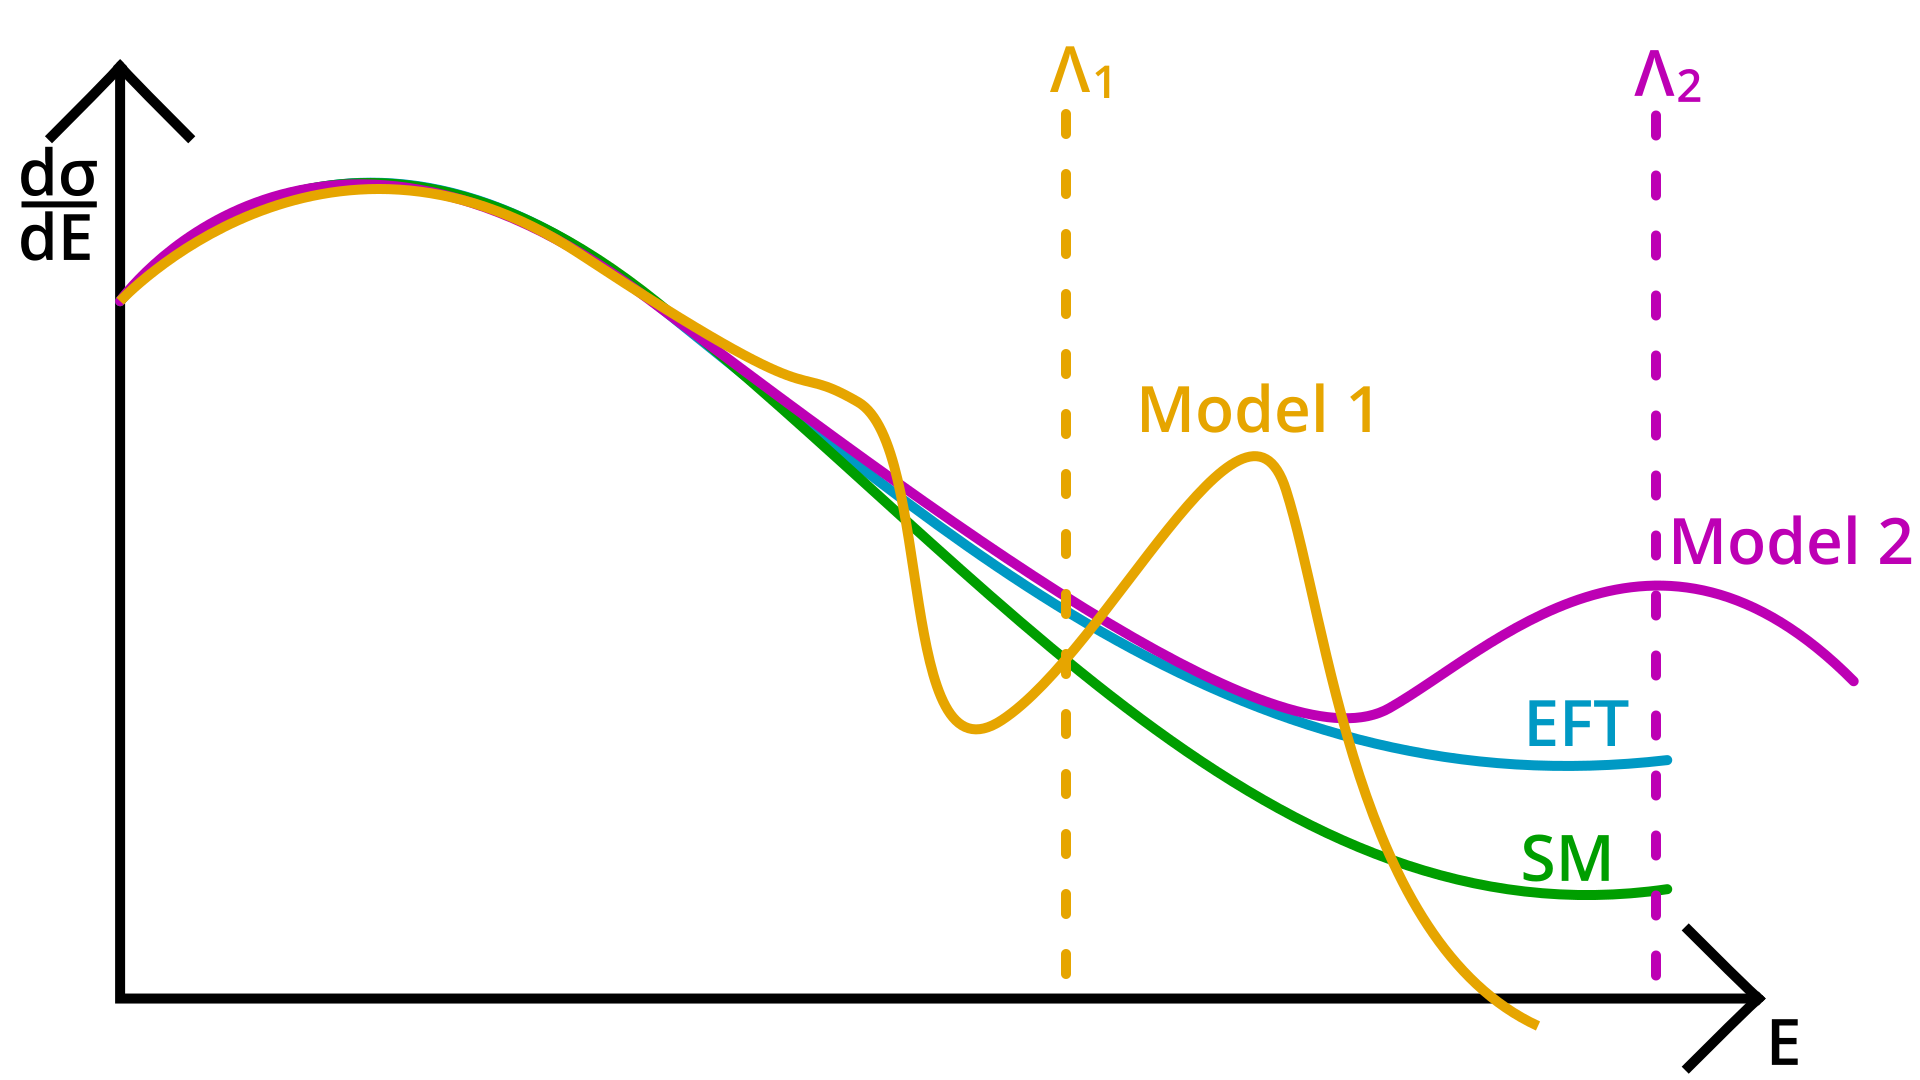
\includegraphics[width=\textwidth]{images/EFT_validity.png}
        \caption{}
    \end{subfigure}
    \begin{subfigure}{0.45\textwidth}
        \centering
        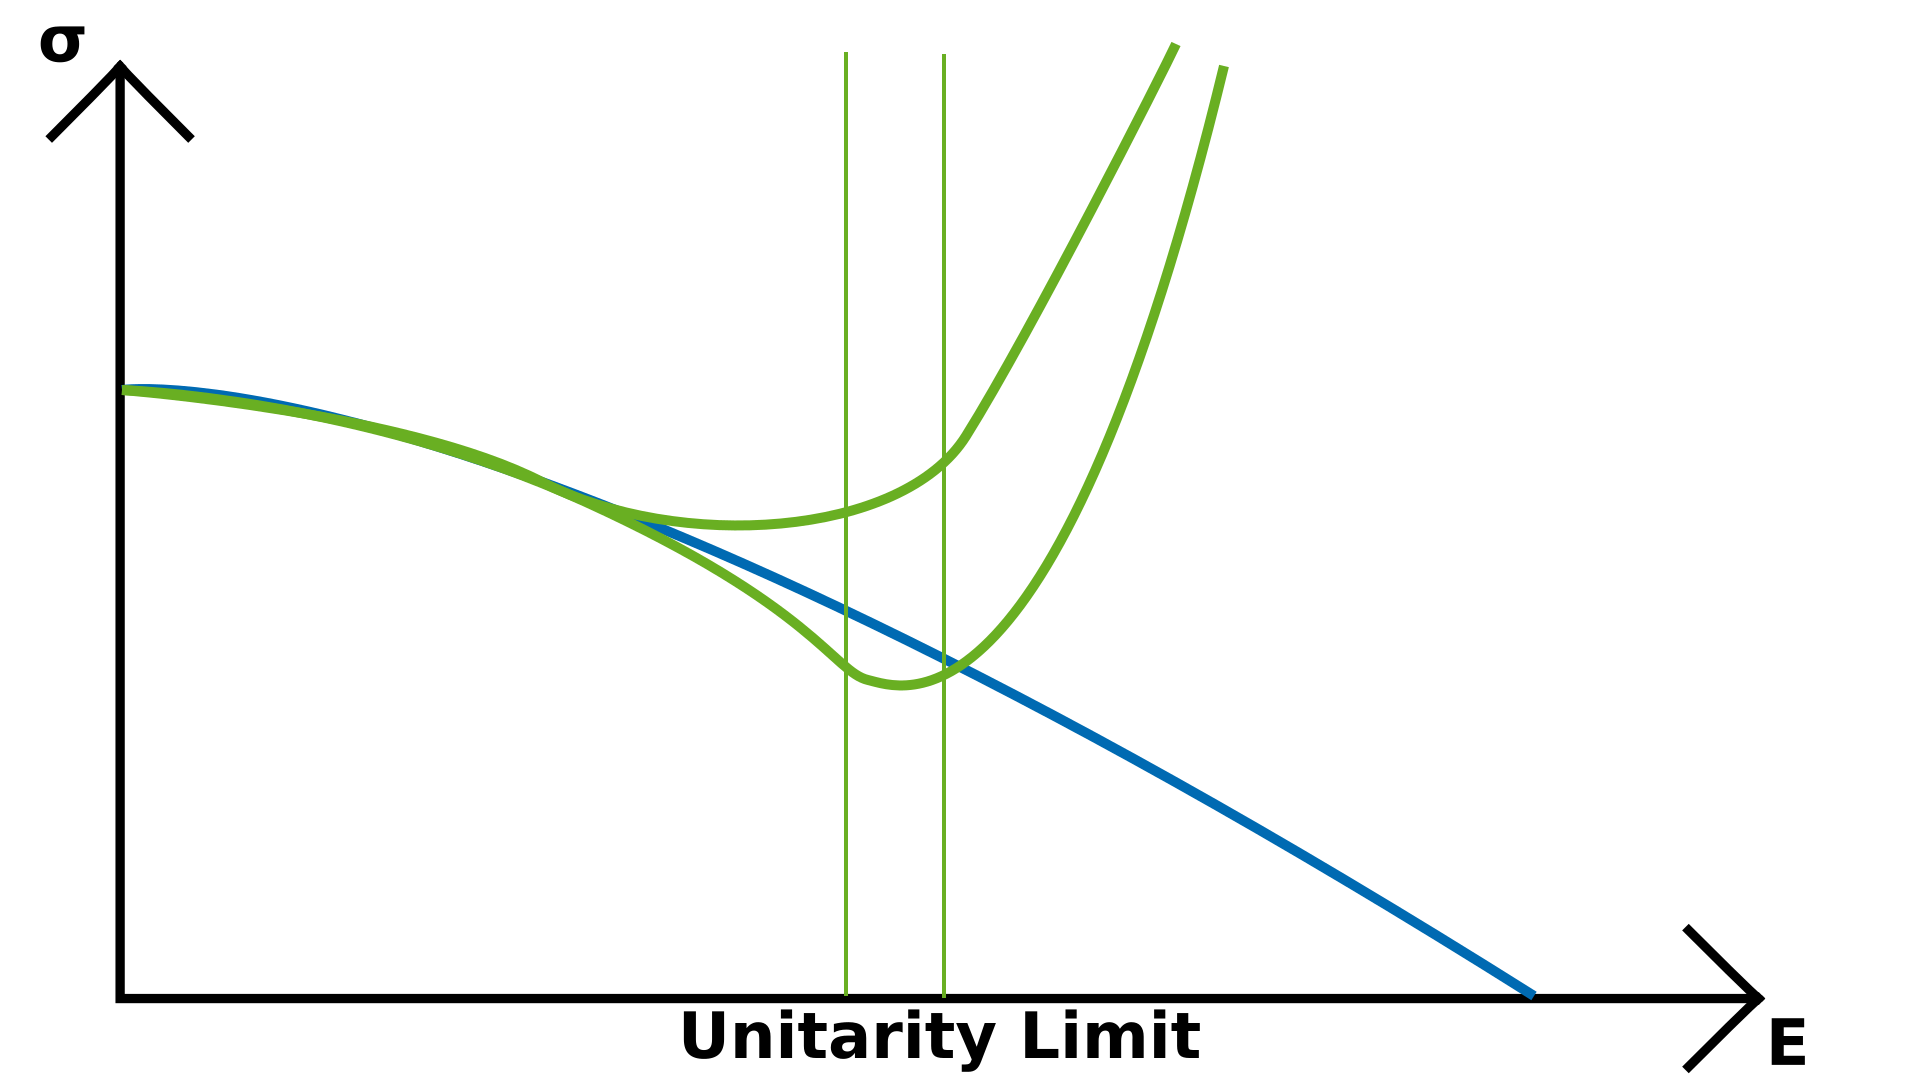
\includegraphics[width=\textwidth]{images/EFT_cross_section.png}
        \caption{}
    \end{subfigure}
    \caption{\textbf{a)} Not all Models can be fitted using EFT only ones with energy scale higher than the SM \textbf{b)} Schematic of unitarity limits the energy range changes depending on the cutoff \cite{MSz} }
    \label{fig:EFT_validity}
\end{figure}
The time evolution of states in quantum mechanics is mathematically described by unitary operators. Time evolution without unitary operators is proposed in new approaches to quantum mechanics like Carl M. Benders talk in 2021 at the TU-Dresden
proposing a quantum theory including non Hermitian Hamiltonian. Unitarity was a decisive concept for the inclusion of the Higgs field in the SM as it restored unitarity at tree level.
EFT isn't a complete theory by extending the SM, TGC and QGC processes are modified leading to unitarity violation. The expected behaviors of a Unitary EFT is dim-6 interference > dim-6 quadratic $\sim$ dim-8 interference > dim-8 quadratic.
This however is not the case as dim-8 operators cause the Scattering amplitude to growth asymptotically $\sim \Lambda^{2}$ eventually leading to unitarity violation \ref{fig:dim8_quad_int_comparission}.
On can now apply a cutoff at the validity scale $M=\Lambda$ but in practice the value of $\Lambda$ is unknown and can only be gained by analyzing data. This means that EFT predictions are only valid for an operator dependent unitarity limit.
It should be noted that unitarity can be restored by using unitarisation. In ATLAS research the relatively simple K-matrix method is commonen tool for unitarisation as shown in \cite{Kilian.2015}. This however does not restore EFT validity and
makes connecting EFT results to UV Theories harder. In conclusion the search for BSM effects using EFT is only possible in an Energy range as light states are not detectable and high Energy states are removed by the unitarity limit \ref{fig:EFT_validity}.
\begin{figure}[h]
    \centering
    \centering
    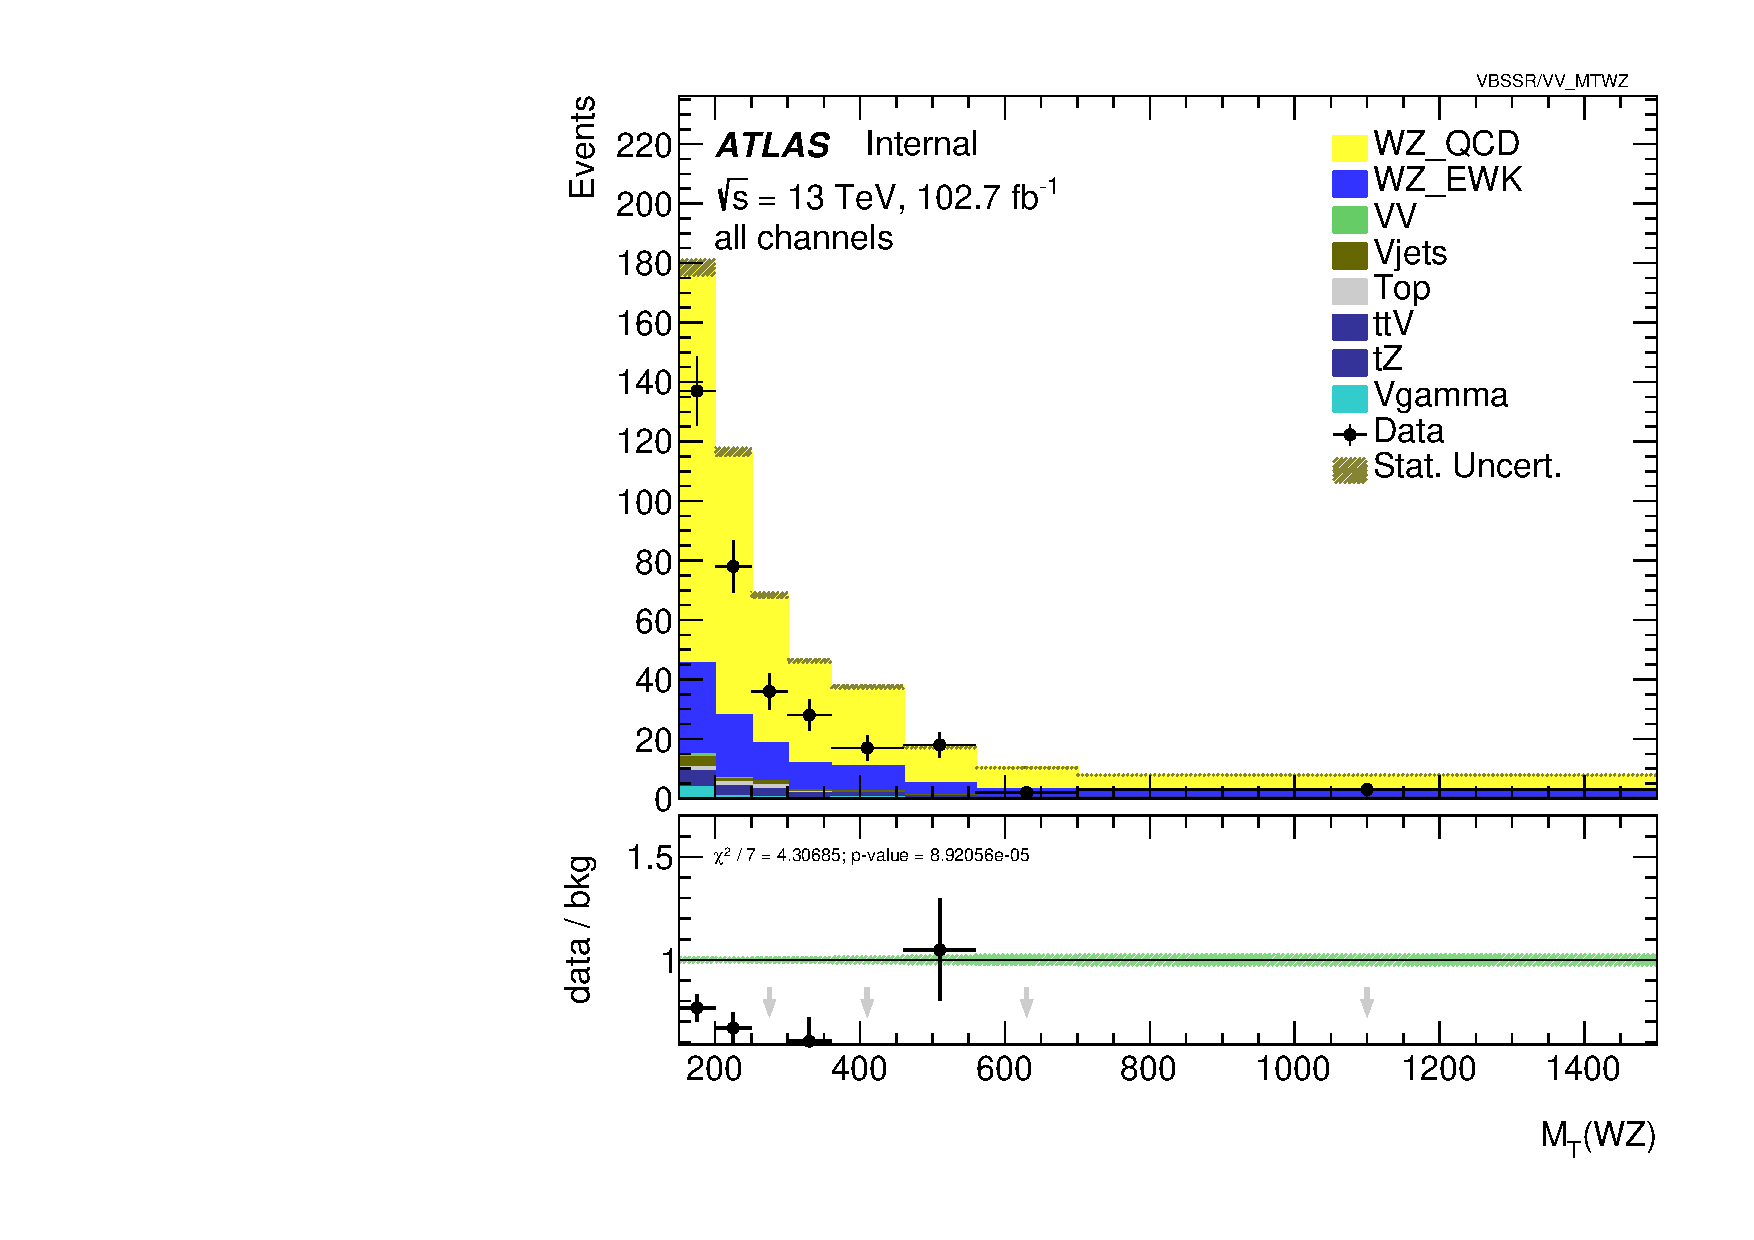
\includegraphics[width=0.45\textwidth]{Plots/Sm_re/all_VV_MTWZ.pdf}
    \caption{Comparission of inteferenz term and quadratic term for the S1 parameters created with value S1=128. The quadratic therm is bigger for higher energies since no unitarisation is used.}
    \label{fig:dim8_quad_int_comparission}
\end{figure}


\end{document}
